\documentclass[11pt]{article}
\usepackage[utf8]{inputenc}
\usepackage[pdftex]{graphicx}
\usepackage{pdfpages}
\usepackage{makeidx}
\usepackage[english]{babel}
\usepackage [autostyle, english = american]{csquotes}
\usepackage{mathtools}
\usepackage{xcolor}
\usepackage{listings}
\usepackage{caption,subcaption}
%\usepackage{subfigure}
\usepackage{geometry}
\usepackage{adjustbox}
\usepackage{calc}
\usepackage{ifthen}
\usepackage{listings}
\usepackage{hyperref}
\usepackage[square,sort,comma,numbers]{natbib}
\usepackage{cleveref}
\usepackage[section,cachedir=build,newfloat]{minted}
\usepackage{chngcntr}
\usepackage[cm]{fullpage}

\definecolor{mintedbackground}{rgb}{0,0,0}


\usemintedstyle{tango}
\newenvironment{code}{\captionsetup{type=listing}}{}
\SetupFloatingEnvironment{listing}{name=Source Code}
\captionsetup[subfigure]{subrefformat=simple,labelformat=simple}

\renewcommand{\thelisting}{\arabic{listing}}
\renewcommand\thesubfigure{(\alph{subfigure})}

\bibliographystyle{abbrvnat}

\geometry{
 a4paper,
 total={170mm,257mm},
 left=20mm,
 top=20mm,
}

\definecolor{lightgray}{rgb}{.7,.7,.7}
\definecolor{gray}{rgb}{.4,.4,.4}
\definecolor{darkblue}{rgb}{0,0,.3}
\definecolor{gray}{rgb}{0.4,0.4,0.4}
\definecolor{darkblue}{rgb}{0.0,0.0,0.6}
\definecolor{cyan}{rgb}{0.0,0.6,0.6}

\lstset{
  basicstyle=\ttfamily,
  columns=fullflexible,
  showstringspaces=false,
  commentstyle=\color{gray}\upshape
}

\lstdefinelanguage{XML}
{
  morestring=[b]",
  morestring=[s]{>}{<},
  morecomment=[s]{<?}{?>},
  stringstyle=\color{black},
  identifierstyle=\color{darkblue},
  keywordstyle=\color{cyan},
  morekeywords={xmlns,version,type}% list your attributes here
}
 
 
\hypersetup{
    colorlinks,
    citecolor=black,
    filecolor=black,
    linkcolor=black,
     urlcolor=black
}
 
\graphicspath{ {images/} }


\newmintedfile[pycode]{python3}{
frame=lines,
framesep=2mm,
fontsize=\footnotesize,
showtabs =false,
autogobble=true,
breaklines=true,
mathescape=true
}

\title{Assignment 1 \\ Introduction to Information Retrieval \\ CS734/834}
\author{John Berlin}
\date{\today}
\renewcommand\thesection{Q.\arabic{section}}
\renewcommand\thesubsection{\thesection}

\begin{document}
\maketitle
\newpage
\section{Question 1.2}
\begin{verbatim}
Site search is another common application of search engines. In this case,
search is restricted to the web pages at a given website. 
Compare site search to web search, vertical search, and enterprise search
\end{verbatim}
\subsection{Answer}
% trim={<left> <lower> <right> <upper>}
To compare the four searches I performed the first three using Google and base query ``async redux". 
The search results shown are limited to the first three in order to have presentable figures.
For the site search I used the site \textit{github.com} as the context for the base query is developing web pages in the React.js ecosystem.
As seen in figure \hyperref[fig:ssearch]{\ref{fig:ssearch}} the results are for libraries that do async actions in redux. The first two is from the redux library itself whereas the third is from a library that enhances that functionality.  \newline

The web searches top three results figure \hyperref[fig:wwwearch]{\ref{fig:wwwsearch}}, featured two results from the online documentation of the library itself and one code example which the first result of the site search.  These results were as expected as the query was missing the context given to search engine through the ``site:github.com" as is done in site search. The context is key when comparing site search to web search as it effects the precision of these queries rather than recall. For example, I made this exact query recently when looking into how to better handle the async problems faced by WAIL\footnotemark \footnotetext{https://github.com/N0taN3rd/wail} which is using flux (the predecessor to redux). I performed the web search first as I wanted to see in the documentation on how redux handled async operations rather than diving into the code bases of the libraries themselves. Google understood the likely hood of this happening for the base query and was precise in its top three results given the lack of context which is present in the site search.
\newline 

Vertical search is done when only results of a certain type are desired which is another contextual based query. The results of this search, using Google Videos figure \hyperref[fig:vsearch]{\ref{fig:vsearch}}, in comparison to the site search can be described as combination of the web search and the site site search. The first two results of this query are a combination of all three results from the web search plus the first and second of the site search. The last result of the vertical search features content from the third result from the site search. 
\newline 

In order to compare enterprise search to site search I will use two examples: the first will be the classical example using my personal computers file search. The second will be using more targeted search on my personal computer within the context of the previous two comparisons. As I do not have a large corporate intranet to search I use \emph{Desktop Search} in this example. Desktop search, as defined in our book, is the personal version of enterprise search \citep[pp. 3]{CroftMetzlerStrohman200902}. I felt this is a correct substitution because the previous two comparisons used examples about how I personally used the them for WAIL. Furthermore if a team of developers was looking to find out where on their computers which libraries are currently being used for async operations figure \hyperref[fig:cdeSearch]{\ref{fig:cdeSearch}} and then where in the repository is the functionality implemented figure \hyperref[fig:tdeSearch]{\ref{fig:tdeSearch}}.

Enterprise Search (\emph{Desktop Search}) returned results that had the search term in them not necessarily the most relevant figure \hyperref[fig:cdeSearch]{\ref{fig:cdeSearch}}. The search term async can be found in directory names as well as many duplicates. The duplicates in these results are a product of the search being done on the file system where duplicates are acceptable. Unlike site search which returned unique results where duplicates are not as common. Whereas if you were to use the Linux utility \emph{grep}, you can perform the same kind of query but limited to lines contained in the files in a specific part of the file system figure \hyperref[fig:tdeSearch]{\ref{fig:tdeSearch}}, much like site search. It is clear to see that enterprise search is a broader type of search yet is done a specific site(file system).
\begin{figure}[h]
	\centering
	\adjustbox{trim={0} {0.5\height} {0} {0},clip}%
	{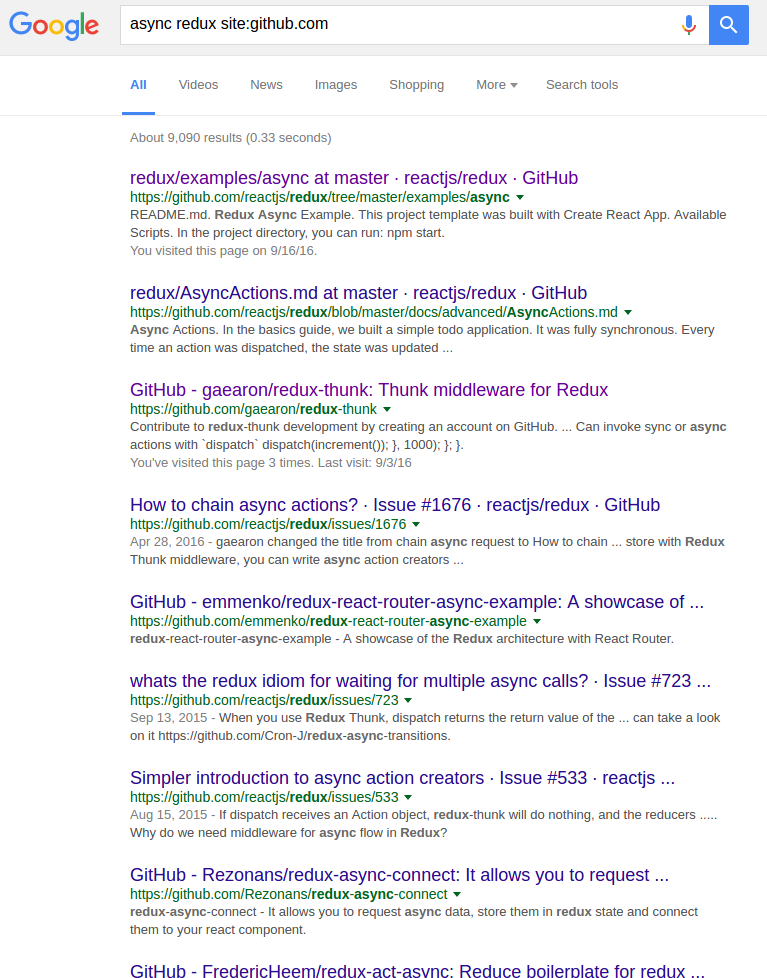
\includegraphics[scale=0.5]{googleSiteSearch.png}}
	\caption{Site Search}
	\label{fig:ssearch}
\end{figure}
\begin{figure}[h]
	\centering
	\adjustbox{trim={0} {0.5\height} {0} {0},clip}%
	{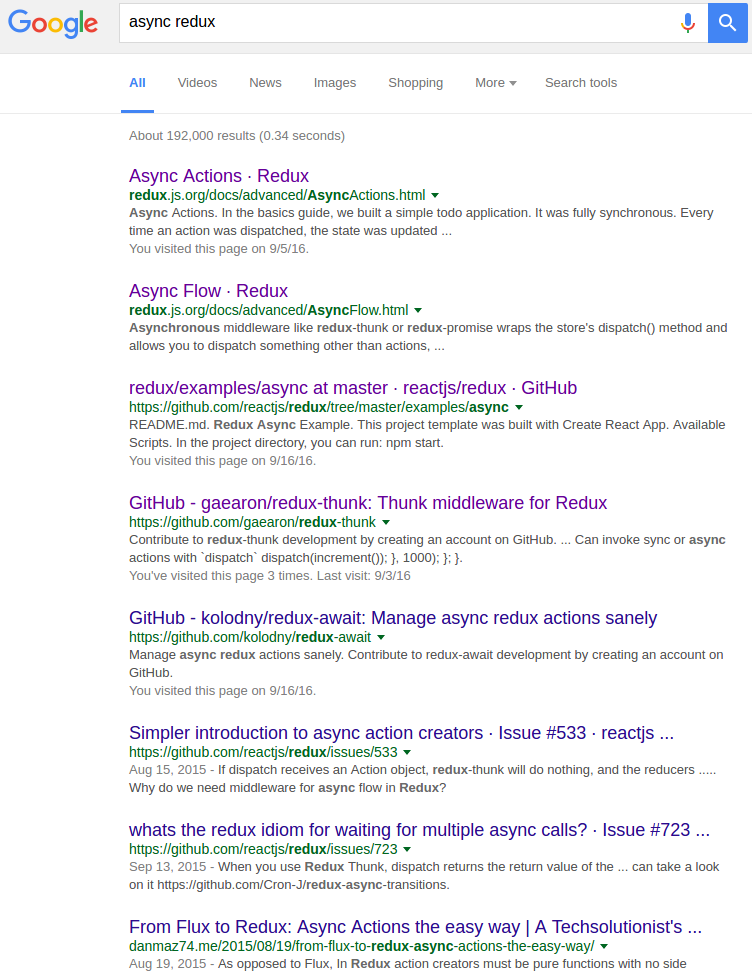
\includegraphics[scale=0.5]{googleWWWSearch.png}}
	\caption{Web Search}
	\label{fig:wwwsearch}
\end{figure}
\begin{figure}[h]
	\centering
	\adjustbox{trim={0} {0.5\height} {0} {0},clip}%
	{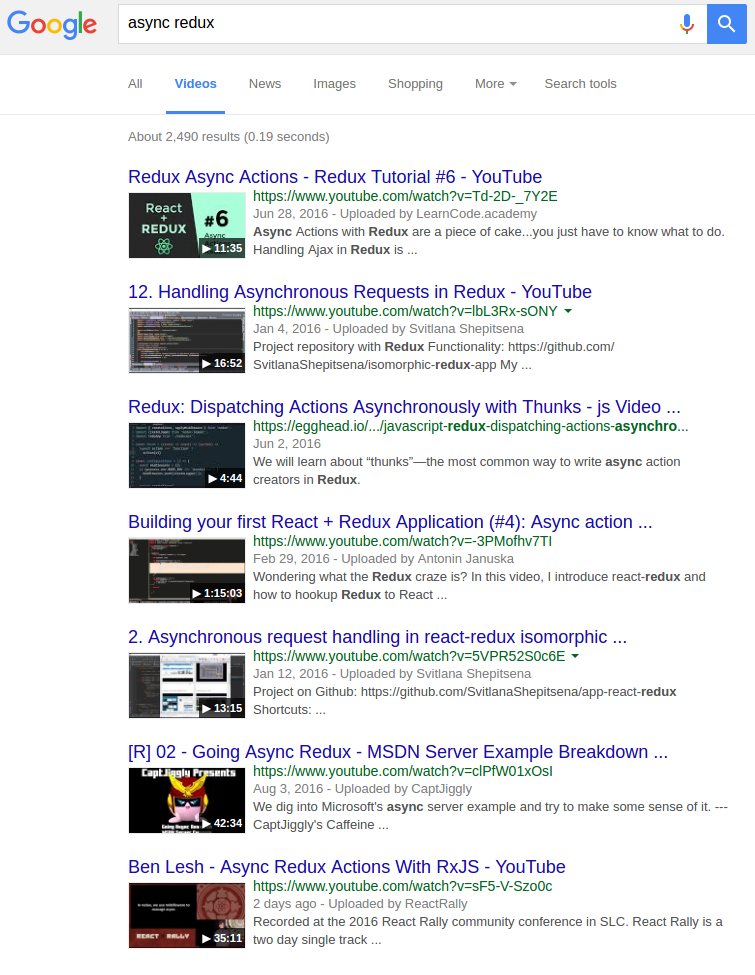
\includegraphics[scale=0.5]{googleVerticalSearch.png}}
	\caption{Vertical Search}
	\label{fig:vsearch}
\end{figure}
\begin{figure}[h]
	\begin{subfigure}{0.45\textwidth}
		\centering
		\adjustbox{trim={0} {0.5\height} {0.3\width} {0},clip}
		{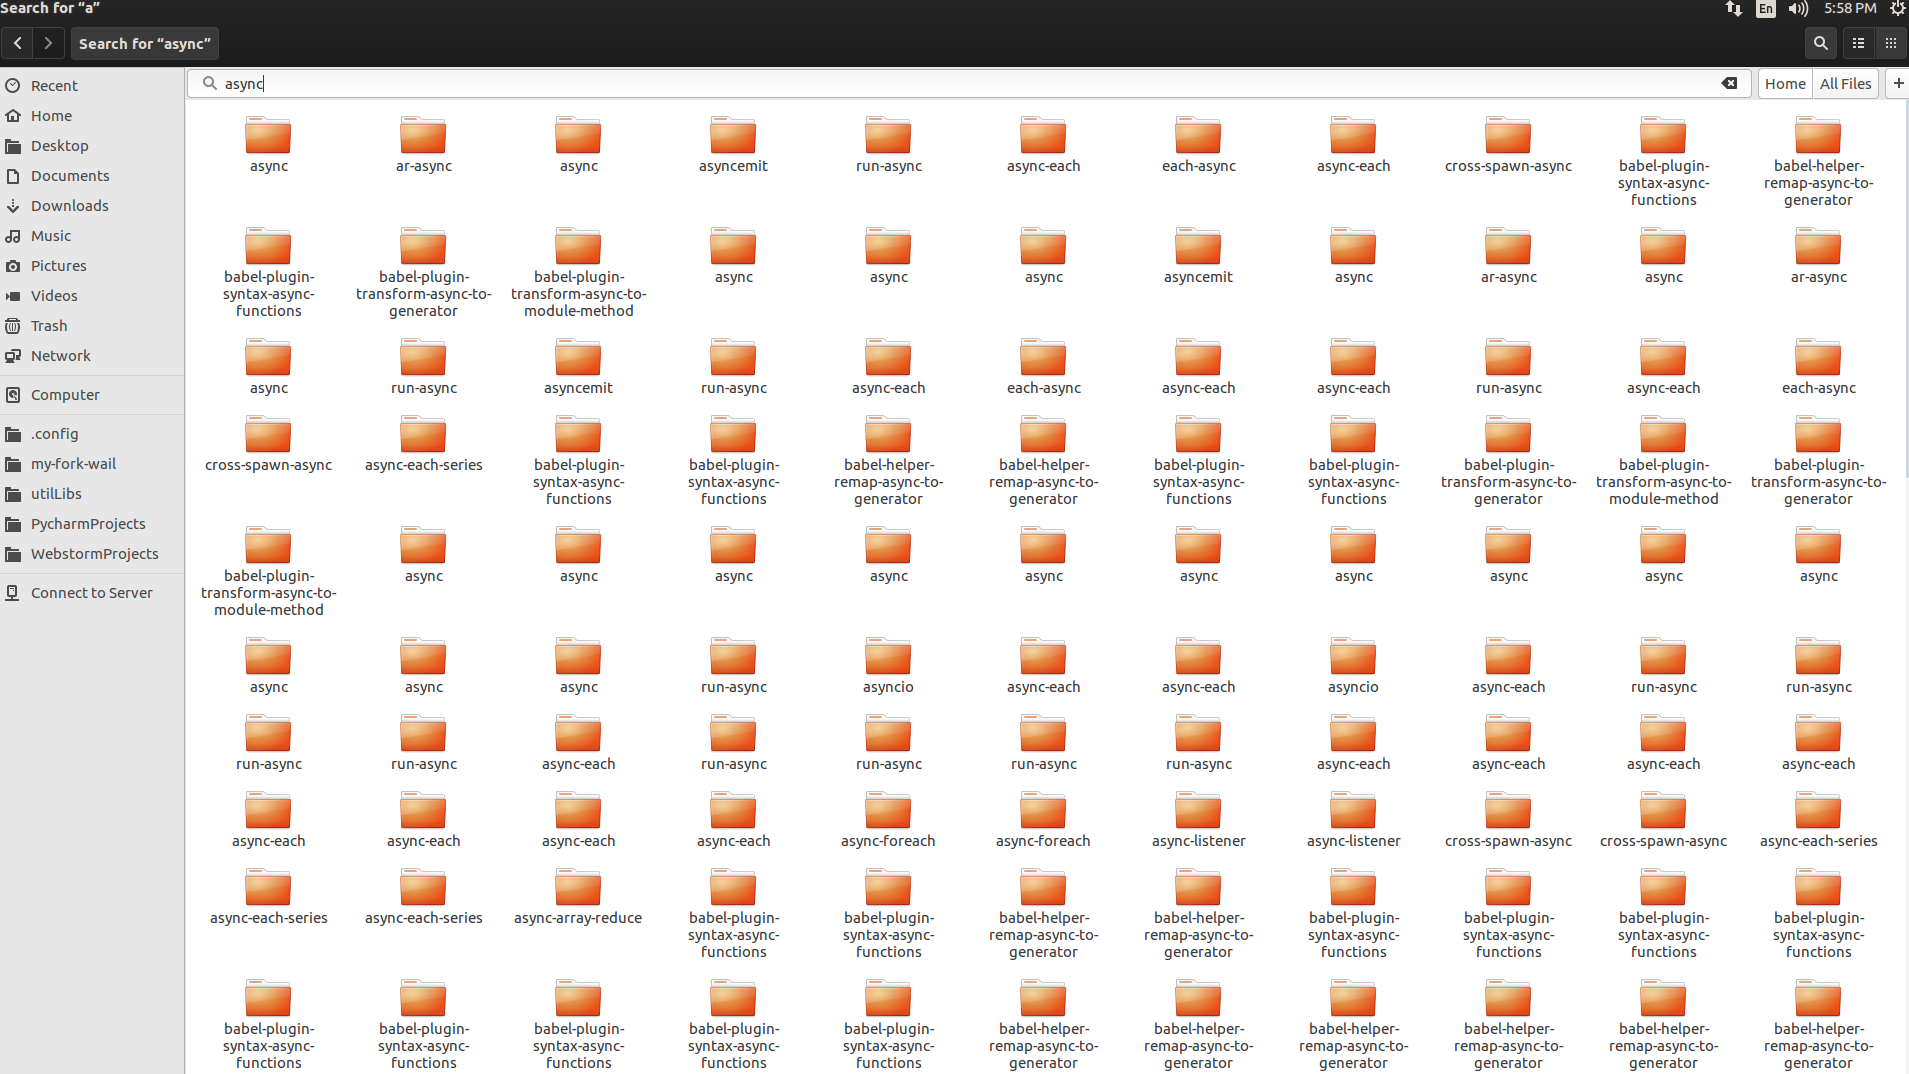
\includegraphics[scale=0.3]{eSearch2.png}}
		\caption{Classic}
		\label{fig:cdeSearch}
	\end{subfigure}
	\vfill
	\begin{subfigure}{0.45\textwidth}
		\centering
		\adjustbox{trim={0} {0.5\height} {0} {0},clip}
		{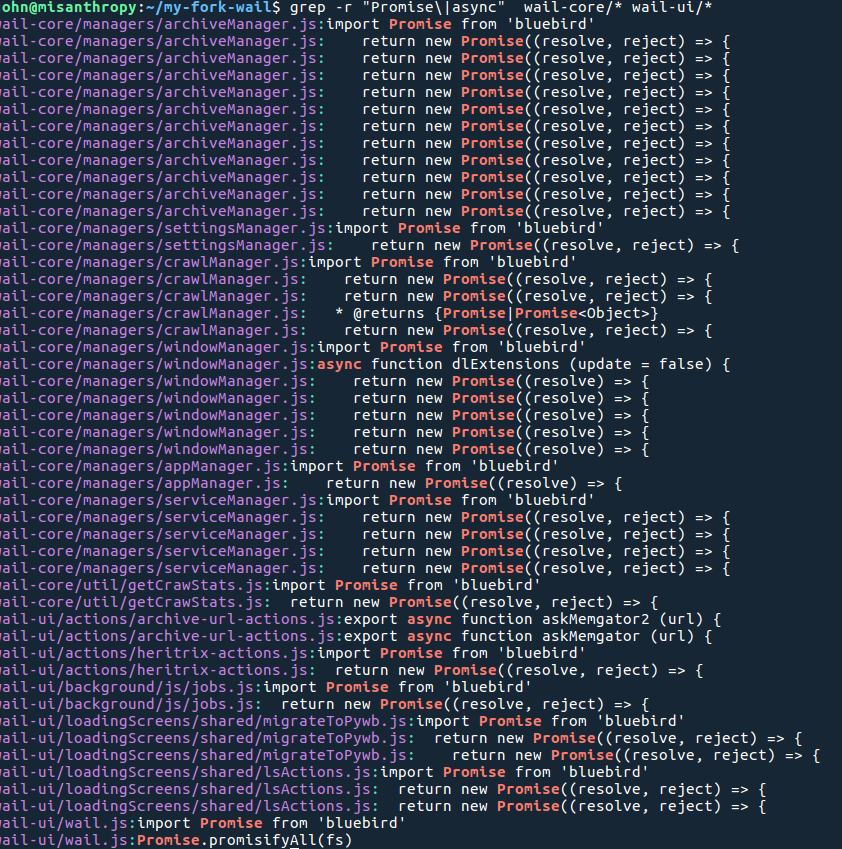
\includegraphics[scale=0.5]{eSearch.png}}   
		\caption{Targeted}
		\label{fig:tdeSearch}
	\end{subfigure}
	\caption{Enterprise (Desktop) Search}
	\label{fig:esearch}
\end{figure}
\newpage
\clearpage
\section{Question 1.4}
\begin{verbatim}
List five web services or sites that you use that appear to use search, not includ-
ing web search engines. Describe the role of search for that service. Also describe
whether the search is based on a database or grep style of matching, or if the search
is using some type of ranking.
\end{verbatim}
\subsection{Answer}
The first website I use that features database style matching is \hyperref[http://www.metal-archives.com/]{metal-archives.com}. Metal archives is a site which allows for you search for a metal band(s) by name, genre, album and many more. You can tell it uses database style search by the search interface it uses and by examining the query string used to produce \autoref{fig:metal}.
\begin{figure}[h]
	\centering
	\adjustbox{trim={0} {0.3\height} {0} {0},clip}
		{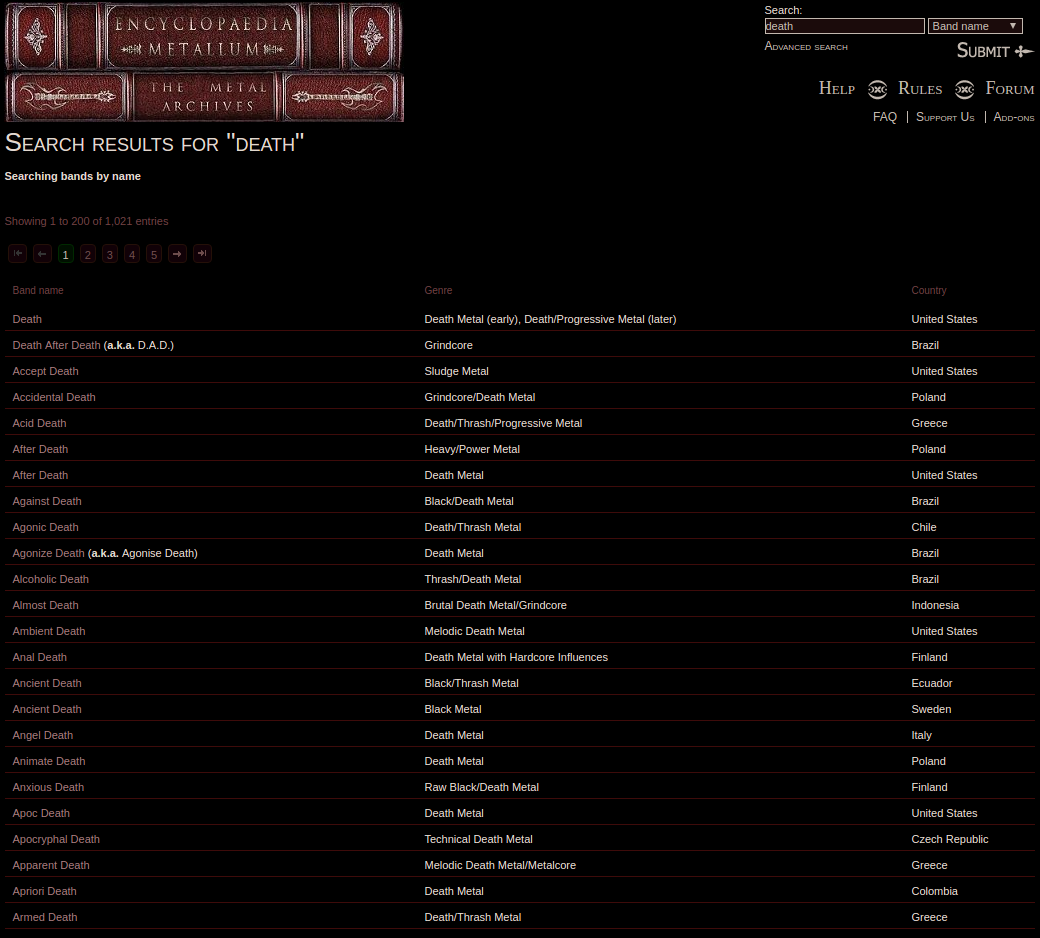
\includegraphics[scale=0.5]{searchStyleMA.png}}  
	\caption{Metal Archives Death} \label{fig:metal}
\end{figure}\newline
The query string ``search?searchString=death\&type=band\_name" shows this site is talking to its REST backend. REST or REpresentational State Transfer is an means to talk to a web service most commonly backed by a database. As seen in \autoref{fig:metal} I am very happy to see that the Floridian death metal pioneers \emph{Death} are at the top of the list for the band name search death. But sadly Stormtrooper of Death (S.O.D) are not in the top results which is a Scott Ian (Anthrax) side project. \newpage
\noindent
The second is \hyperref[https://github.com]{github} which features a mix of database search with grep style searching. \autoref{fig:git} shows the result of search for quick sort on github. The default search results are repositories with the search terms contained in there name and or in the Readme.md contained in the repo itself hence grep. Along with the repository search you can also search code i.e code lines for the presence of your search terms.  Further solidifying the declaration of mixed is the ability to do ``git grep" to search for a term across all branches in your repository and that the query string used to produce \autoref{fig:git} ``search?utf8=\%E2\%9C\%93\&q=quick+sort" indicates another RESTful style web api.

\begin{figure}[h]
	\centering
	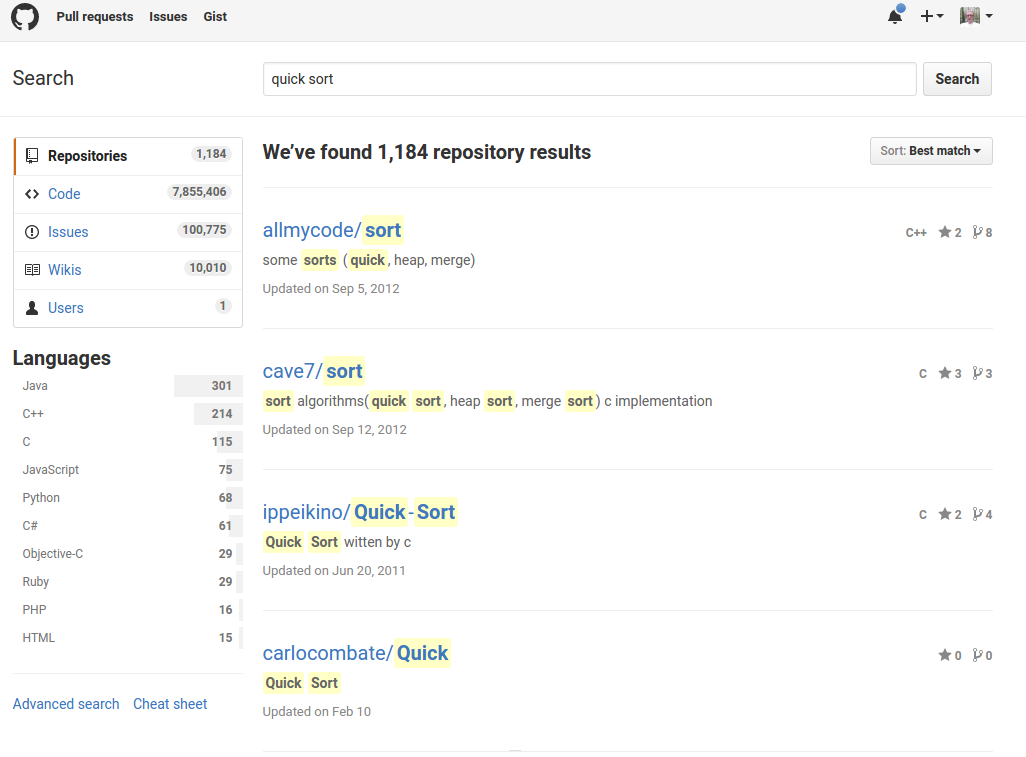
\includegraphics[scale=0.5]{searchStyleGH.png}
	\caption{Github Quick Sort} \label{fig:git}
\end{figure}
\newpage
\noindent
\hyperref[https://www.npmjs.com]{npmjs.com} is another service I use to look when looking for Nodejs packages. \autoref{fig:npm} shows the results when searching for react packages which produces the query string search?q=react. Npmjs.com is the web site for npm, node package manager, which is a service that manages node libraries much like github. It is clear to see that npmjs.com is database search.
\begin{figure}[h]
	\centering
	\adjustbox{trim={0}  {0} {0.1\width} {0},clip}
		{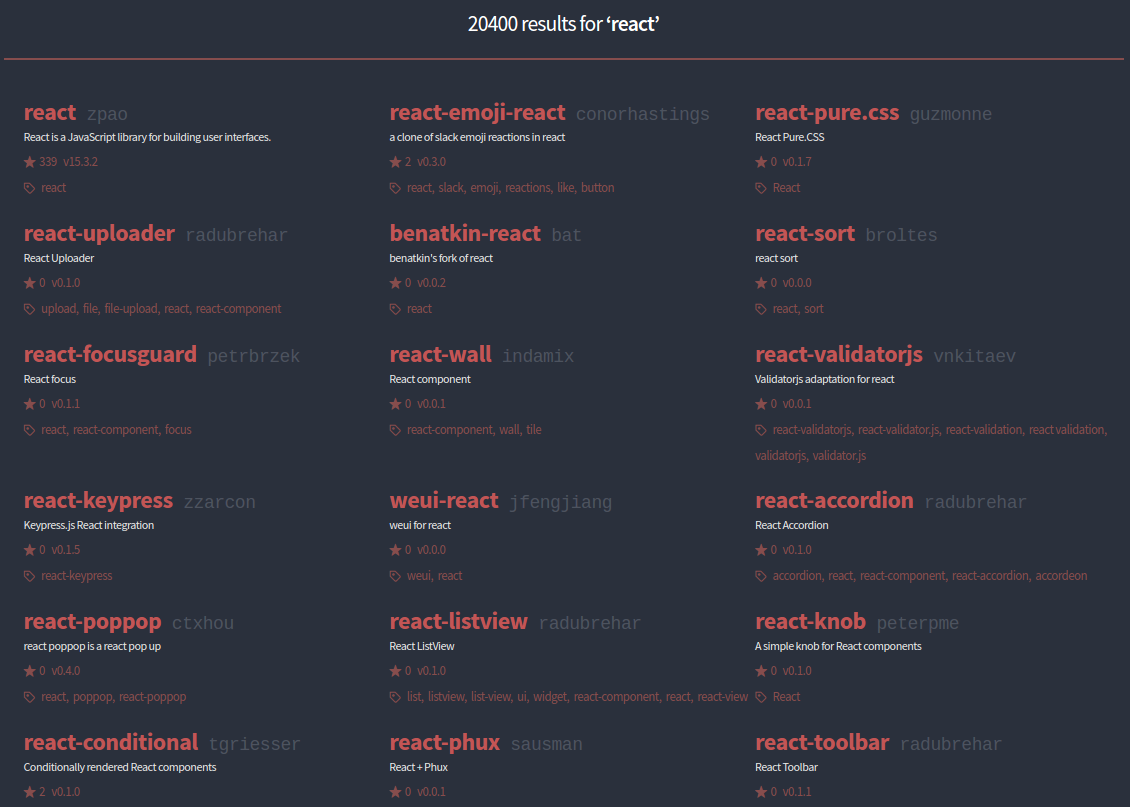
\includegraphics[scale=0.5]{searchStyleNPM.png}} 
	\caption{NPM React} \label{fig:npm}
\end{figure}
\newpage
\noindent
Another database style searched website I use is \hyperref[http://tex.stackexchange.com]{tex.stackexchange.com} which features the power of stackoverflow but for \LaTeX related issues. \autoref{fig:tex} shows the results when searching for questions tagged with bibliographies sorted by frequency. The query string that goes along side this search is
``questions/tagged/bibliographies?sort=frequent" and once again indicates the search was executed against a database.
\begin{figure}[h]
	\centering
	\adjustbox{trim={0}  {0} {0.1\width} {0},clip}
		{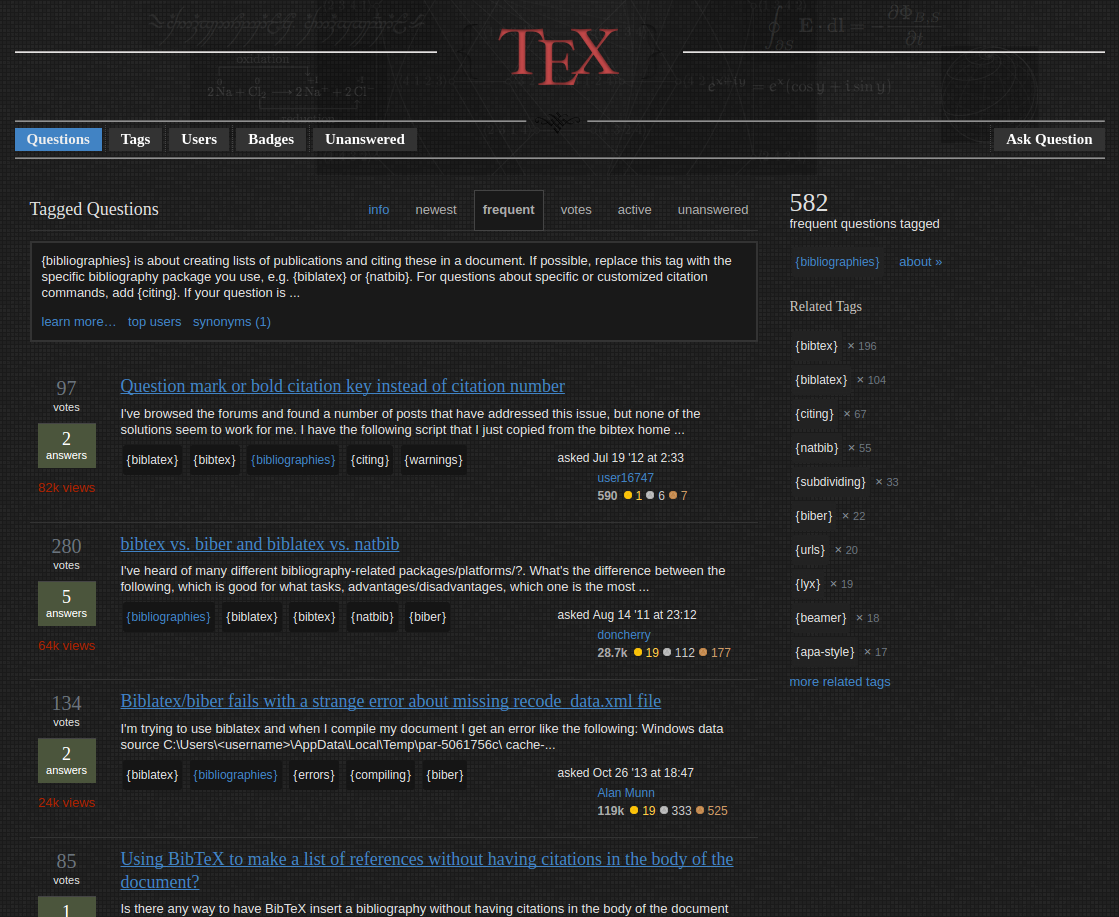
\includegraphics[scale=0.5]{searchStyleTex.png}} 
	\caption{Tex Stack Exchange Bibliographies} \label{fig:tex}
\end{figure}
\newpage
\noindent
Finally my most frequented and favorite database probably grep search style website \hyperref[https://bandcamp.com/]{bandcamp}. \autoref{fig:powerviolence} shows the results when searching for my favorite sub-genre of punk which is power violence. The query string that accompanies this result is ``tag/power-violence".  The results of this query are somewhat disappointing as the band ACxDC dominates the results. They are not a bad band but are the like the Metallica of power violence but eclipse bands like Chiens, whose only recognition in the top results is the split with ACxDC. Great bands like Insect Warfare and Apartment 213 still made it in the top results tho. But the greatest sadness in this is that the power violence powerhouse Gets Worse is no where to be seen. They have been pumping out eps at a steady rate since 2012 all of which blow away ACxDC in terms of the ferocity of their raw and gritty sound continually perfected with each release. 

\begin{figure}[h]
	\centering
	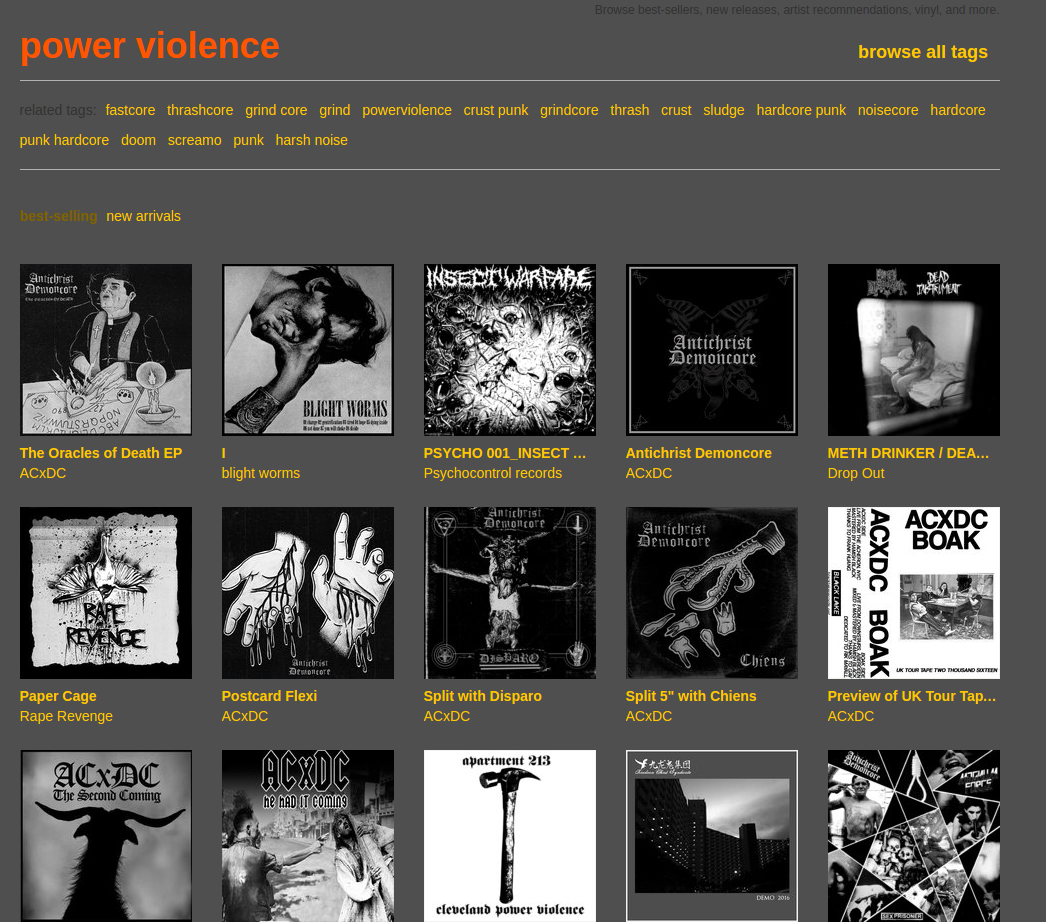
\includegraphics[scale=0.5]{searchStyleBC.png}
	\caption{Bandcamp Power Violence} \label{fig:powerviolence}
\end{figure}






\newpage
\clearpage
\section{Question 3.7} \label{sec:q2}
\begin{verbatim}
Write a program that can create a valid sitemap based on the contents of a
directory on your computer’s hard disk. Assume that the files are accessible from
a website at the URL http://www.example.com . For instance, if there is a file in
your directory called homework.pdf , this would be available at http://www.exam-
ple.com/homework.pdf . Use the real modification date on the file as the last modi-
fied time in the sitemap, and to help estimate the change frequency.
\end{verbatim}
\subsection{Answer}
\setcounter{listing}{0}
The code for this question can be seen in the source code listing \hyperref[code:sitemap]{\ref{code:sitemap}}. The programs utilizes three libraries which made this question easy: PyFilesystem \cite{pyfs} for its combination of listing the contents of a directory and file stats in a single function call, Arrow \cite{arrow} the python version of Momentjs and Yattag\cite{yattag} pythonic document creation. Using pythons argument parser library to get the directory for which to create the sitemap, the program lists the contents of the directory and if the name of the file is acceptable, determined by ``-dots" (include . files or not) argument create a new xml node were the last modified time is converted into utc and finally after the files of the direct have been read output the created site to stdout.  \autoref{sitemap} shows the output of code listing \hyperref[code:sitemap]{\ref{code:sitemap}} when run on a directory containing the wiki for WAIL.
\begin{lstlisting}[language=xml, frame=single, caption={Sitemap of the Wiki for WAIL}, label=sitemap]
<urlSet xmlns="http://www.sitemaps.org/schemas/sitemap/0.9">
  <url>
    <loc>http://www.example.com/Using+Wail.md</loc>
    <lastmod>2016-08-03T03:32:46.439265+00:00</lastmod>
  </url>
  <url>
    <loc>http://www.example.com/Home.md</loc>
    <lastmod>2016-08-03T03:10:43.711074+00:00</lastmod>
  </url>
  <url>
    <loc>http://www.example.com/Getting+Started.md</loc>
    <lastmod>2016-08-03T03:38:06.393983+00:00</lastmod>
  </url>
  <url>
    <loc>http://www.example.com/Screen-Shots.md</loc>
    <lastmod>2016-08-03T00:59:45.379063+00:00</lastmod>
  </url>
  <url>
    <loc>http://www.example.com/FAQ.md</loc>
    <lastmod>2016-08-03T00:59:45.379063+00:00</lastmod>
  </url>
  <url>
    <loc>http://www.example.com/images/misc.png</loc>
    <lastmod>2016-08-02T18:40:20+00:00</lastmod>
  </url>
  <url>
    <loc>http://www.example.com/images/wailSideBar.png</loc>
    <lastmod>2016-08-02T18:38:14+00:00</lastmod>
  </url>
  <url>
    <loc>http://www.example.com/images/services.png</loc>
    <lastmod>2016-08-02T18:40:04+00:00</lastmod>
  </url>
  <url>
    <loc>http://www.example.com/images/frontpage.png</loc>
    <lastmod>2016-08-02T18:38:48+00:00</lastmod>
  </url>
  <url>
    <loc>http://www.example.com/images/heritrixRunningCrawlOptions.png</loc>
    <lastmod>2016-08-02T18:41:04+00:00</lastmod>
  </url>
  <url>
    <loc>http://www.example.com/images/wayback.png</loc>
    <lastmod>2016-08-02T18:39:04+00:00</lastmod>
  </url>
  <url>
    <loc>http://www.example.com/images/configureNewCrawl.png</loc>
    <lastmod>2016-08-02T18:39:44+00:00</lastmod>
  </url>
  <url>
    <loc>http://www.example.com/images/heritrix.png</loc>
    <lastmod>2016-08-02T18:39:22+00:00</lastmod>
  </url>
  <url>
    <loc>http://www.example.com/images/settings.png</loc>
    <lastmod>2016-08-02T18:40:44+00:00</lastmod>
  </url>
</urlSet>
\end{lstlisting}
\begin{code}
	\pycode{code/siteMap.py}
	\captionof{listing}{Python Directory Sitemap Generation} \label{code:sitemap}
\end{code}
\newpage
\clearpage
\section{Question 3.9}
\begin{verbatim}
Write a simple single-threaded web crawler. Starting from a single input URL
(perhaps a professor’s web page), the crawler should download a page and then
wait at least five seconds before downloading the next page. Your program should
find other pages to crawl by parsing link tags found in previously crawled docu-
ments.
\end{verbatim}
\subsection{Answer}
\setcounter{listing}{1}
The solution to this question is a modified version of the solution submitted for assignment 1 for cs532 and the source can be seen in source code listing \hyperref[code:crawler]{\ref{code:crawler}}.
The modifications made to the original were minor instead of looking for links that resolve to pdf files the code now extracts all links from a uri that resolves to a 200 and puts them into a queue the frontier\_gen function. 
The first uri or seed is placed in the queue first and the first call to frontier\_gen is made. Then after waiting for five sections the next uri is popped from the queue and the links contained in it are added. I have added an additional part to this assignment which is a stopping criteria hops. Hops is the number links away from seed url and the reason for this stipulation can be seen in figure \hyperref[fig:frontierSize]{\ref{fig:frontierSize}}. After the first hope the frontier has reached a size of 2833 uris waiting to be processed after visiting links one hope away from the seed url http://cs.odu.edu/$\sim$mln. I also did this from experience gained while working with Heritrix which will download the entire internet if it is not given explicit hop bounds.
The current hop the program is at is determined by decrementing the frontier count gotten at the start of next hop by taking the length of the queue. When it reaches zero the last uri for the final\_hop has its links extracted and the remaining uris are printed. 
\begin{figure}[h]
	\centering
	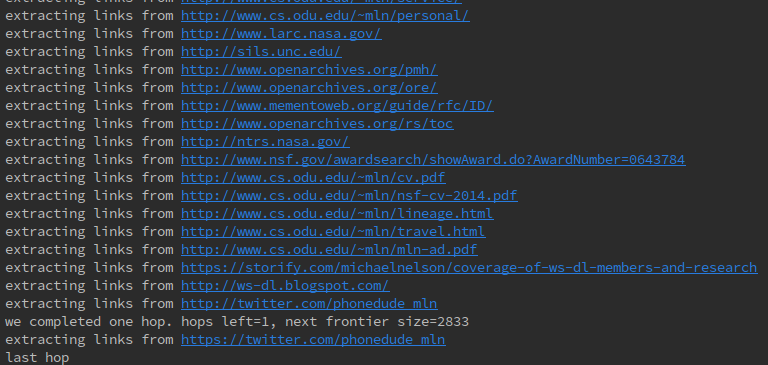
\includegraphics[scale=0.5]{crawlerOutput.png}
	\caption{Frontier Size} \label{fig:frontierSize}
\end{figure}
\begin{code}
	\pycode{code/crawler.py}
	\captionof{listing}{Python Single Threaded Crawler}
	\label{code:crawler}
\end{code}
\newpage
\clearpage
\section{Question 3.14}
\begin{verbatim}
Write a program to generate simhash fingerprints for documents. You can
use any reasonable hash function for the words. Use the program to detect du-
plicates on your home computer. Report on the accuracy of the detection. How
does the detection accuracy vary with fingerprint size?
\end{verbatim}
\subsection{Answer}
\setcounter{listing}{2}
In order to answer this question I used six files with following naming scheme: \emph{name.ext}, \emph{not\_name.ext} and \emph{name\_same.ext}. The first set of three used the syllabus for this course for the base and similar files with the not similar file being the assignment description for websci assignment 1. The second set uses the \LaTeX \ source submitted for websci assignments 1 and 9. The second set's base and same file is assignment 9 source and the not similar file is the source for assignment 1. These files can be found in the directory \emph{simularDocs} which accompanies this report. \newline

\noindent
The hashing function used for the words or tokens as I refer to them in \autoref{code:simhash} is md5. Md5 is used as it has the property of given an input it will produce the same hash on consecutive usage of the function on the same input. Before calculation of the hash for each token the documents text was sanitized by removing the punctuation and tokens that were found to be in a stop word list provided by \textit{NLTK} \cite{nltk} or less than two characters long. For all tokens that passed the filtering criteria their weights were calculated as the frequency in which they appeared, for example if a token appeared in the document twice it was assigned the the weight of two. After the token weights were calculated each of the tokens were hashed. Md5 in python can return the digest of the hash in two forms: the digest itself or an hexadecimal representation of the digest. The hex digest was used as it is the quickest to transform into a binary string. The conversion from hex to binary is as follows: for each character in the hexadecimal representation of the digest, determine its ordinal value and represent it as a binary value.\newline

\noindent
Three cases were used to test the effectiveness of this implementation of simhash. The first used a bit length of 8  which was used in the example found in the book \citep[pp. 64]{CroftMetzlerStrohman200902} as a base line. The results \autoref{fig:shb8} show that simhash was able to determine the duplicates syllabus\_same.txt, syllabus.txt and websci\_assignemnt9.tex, websci\_assignemnt9\_same.tex  both of which had similarity scores of $1.0$. The duplicates in this test when compared to the ``same" files both had scores of  $0.8944$. This seems odd but will be explained in the next test.
\begin{figure}[h]
\centering
	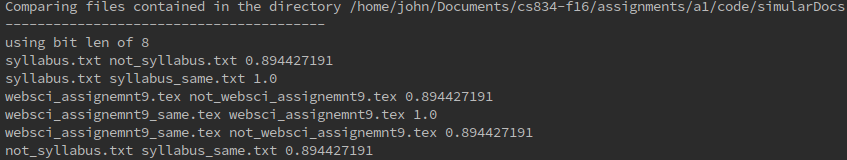
\includegraphics[scale=0.6]{simhashB8.png}
	\caption{Simhash simularity using bit length of 8} \label{fig:shb8}
\end{figure}\newline
The second test used the minimum length of the bit string produced over all terms by md5. \autoref{tb:md5lens} shows the maximum hash length produced by md5 for a document to help get an idea of the size of the hashes when considering it's role in the similarity calculations.
\begin{table}[h]
\centering
\begin{tabular}{|l|l|}
\hline
\multicolumn{1}{|c|}{file} & \multicolumn{1}{c|}{max hash length} \\ \hline
websci\_assignemnt9.tex & 213 \\ \hline
not\_websci\_assignemnt9.tex & 213 \\ \hline
syllabus.txt & 210 \\ \hline
not\_syllabus.txt & 211 \\ \hline
\end{tabular}
\caption{Max bit length of terms produced by md5}
\label{tb:md5lens}
\end{table}\newline
As seen in table one the lengths of the hash can get large. Which in turns leads to the conclusion to be that the differences in the hashes must not be in the most significant bits in the binary representation of the hash. It must be noted that since the \LaTeX \ files used share markup terms this would lead to them having similar maximum hash lengths even after punctuation has been removed. To compensate for this case the minimum hash length was used for the number of bits in the similarity computation as seen in  \autoref{fig:shmd5}.
\begin{figure}[h]
\centering
	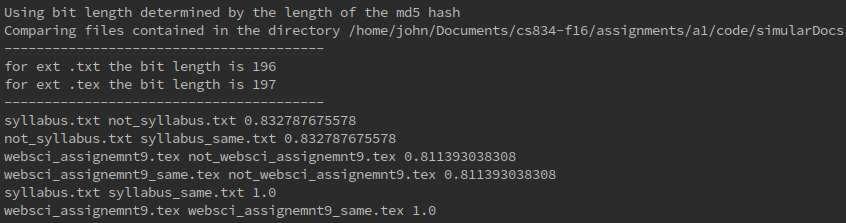
\includegraphics[scale=0.6]{simhashMD5.png}
	\caption{Simhash simularity using min md5 length} \label{fig:shmd5}
\end{figure}\newline
The minimum hash length is close to for both document types $196$ syllabus and $197$ websci but the similarities for the non-similar files are more distance at $0.8327$ and $0.8113$ respectively. This confirms the assumption that the significant digits of the hash do not play as great of a role for large hash lengths.
The final test uses the random value generated as describe previously with lower bounds of $10$ and upper bound of $20$, the results are seen in \autoref{fig:shrandy}. Once again the significant bits come into play with the similarity between non-similar files. The syllabus files were the only group to have the distinction made for different files with score of $0.875$ whereas the websci files no difference could be determined.
\begin{figure}[h]
\centering
	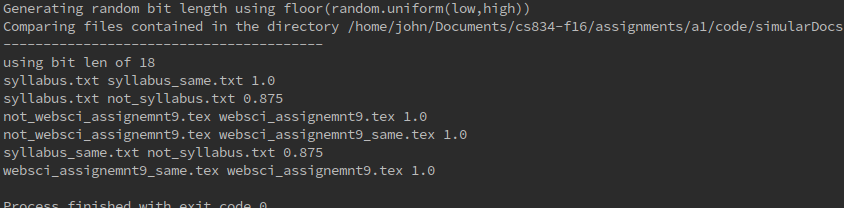
\includegraphics[scale=0.6]{randBits.png}
	\caption{Simhash simularity using random bits} \label{fig:shrandy}
\end{figure}\newline
\begin{code}
	\pycode{code/docSimhash.py}
	\captionof{listing}{Simhash Generator and Document Similarity}
	\label{code:simhash}
\end{code}
\newpage
\clearpage
\bibliography{refrences}

\end{document}